\documentclass[12pt]{article}
\usepackage{myart}
\usepackage[english]{babel}
\usepackage[ruled,vlined,linesnumbered]{algorithm2e}
\usepackage[center]{titlesec}
\renewcommand{\refname}{REFERENCES}
% \renewcommand{\contentsname}{REFERENCES}
\titlelabel{\thetitle.\quad}
\newcommand{\sectionbreak}{\clearpage}
\let\originalparagraph\paragraph
\renewcommand{\paragraph}[2][.]{\originalparagraph{#2#1}}
\titleformat{\section}[block]{\Large\bfseries\filcenter}{\thesection.\;}{0.1em}{\uppercase}

\titleformat{\subsection}[block]{\large\bfseries\filcenter}{\thesubsection.\;}{0.1em}{}
\titleformat{\subsubsection}[block]{\bfseries\filcenter}{\thesubsubsection.\;}{0.1em}{}
% \renewcommand{\rmdefault}{ftm}
%\usepackage{hyperref}
%\newcommand{\dG}{\Delta G}
%\newcommand{\TdS}{T \Delta S}
%\newcommand{\br}{\mathbf{r}}
\graphicspath{ {fig/} }
\newcommand\undermat[2]{%
  \makebox[0pt][l]{$\smash{\underbrace{\phantom{%
    \begin{matrix}#2\end{matrix}}}_{\text{$#1$}}}$}#2}
\begin{document}

\pagenumbering{arabic}
\clearpage

\setcounter{page}{3}
\begin{center}
	Structured learning for model generation\\
	Artem Bochkarev \\[5mm]
	Submitted to the Skolkovo Institute of Science and Technology
	on 01 June 2018 \\[5mm]
	\textbf{ABSTRACT:}
\end{center}

% \\[5mm]
Skoltech Research Advisor: \\
Name: Maxim Fedorov \\
Degree: Professor \\
Title: Director, CREI CDISE \\[5mm]
MIPT Research Advisor: \\
Name: Vadim Strijov \\
Degree:{\color{red} TO DO} \\
Title: {\color{red} TO DO}

\newpage

\tableofcontents

\section{Introduction}
Genetic programming \cite{koza1992genetic} is a powerful approach for building models.
Symbolic regression \cite{zelinka2005analytic} uses genetic algorithms \cite{davis1991handbook} in order to find the mathematical expression for the optimal approximation model.
The resulting model is interpretable and understandable by experts in the application field \cite{johnson2000explanatory}.
The other advantage of genetic programming is that it provides very high quality of approximation. Genetic algorithms often outperform other optimization methods in complex and multimodal problems \cite{moles2003parameter}.

These advantages make genetic programming suitable for many applications.
Symbolic regression is used for ranking documents upon user request in information retrieval \cite{kulunchakov2017generation}, for classification of time series of physical measurements \cite{eads2002genetic} and for diagnosing pathologies from medical data \cite{tsakonas2004evolving}. It was also shown that genetic programming can improve optimization of deep neural networks \cite{david2014genetic}.

The main drawback of genetic approach is that it is guided random search, therefore in some circumstances it might be very slow due to improper selection of heuristics.
The problem is addressed in \cite{li2016accelerated} using acceleration on GPU.
The goal of this study is to increase the speed of generating models in the form of mathematical expressions.

The proposed method is based on meta learning approach.
The thorough relevant survey of the field is presented in \cite{lemke2015metalearning, brazdil2018metalearning}.
The aim is to find an optimal model for a new approximation problem (base problem), given the optimal models for previous similar base problems.
Each mathematical expression is seen as a binary tree of superpositions of primitive functions.
The model in this case is a tree and the problem is to learn to predict a complex structure.
The overview of structured learning approaches can be found in \cite{nowozin2011structured}.
The problem can also be posed as decoding tree structure from some vector representation of base problem.

In \cite{jin2018junction} authors propose tree autoencoder architecture for generating structures of the molecules. In the paper \cite{parisotto2016neuro} the model for generating programs from input-ouput pairs is proposed.


\newpage

\section{Problem Statement}
Consider the set of supervised problems with optimal models for them.
Each single supervised problem is named ``base problem''.
The regression problems are considered to be base problems in this study.
The model for a base problem is a mathematical expression.
The goal of this study is to build a method to find models for base problems automatically.

\subsection{Base problem}
\label{base}
Denote $\mathbf{X} = \{\mathbf{x}_i\}_{i=1}^n \in~\mathbb{R}^{n \times l}$ be the feature matrix and $\mathbf{y} = \{y_i\}_{i=1}^n$ be the vector of target variables for the base problem.
The feature matrix $\mathbf{X}$ and target vector $\mathbf{y}$ are combined into the dataset $D = (\mathbf{X}, \mathbf{y})$ which is a full description of a base problem.
From now on we denote both base problem and its dataset as $D$.

In this study the following conditions are posed to the base problem:
\begin{itemize}
	\item $\mathbf{x}_i$ is not random,
  \item $\{\mathbf{x}_i\}_{i=1}^n$ is an ordered set,
  \item $\mathbf{y}$ is random,
	\item $\exists f: y_i = f(\mathbf{x}_i) + \varepsilon_i$,
  \begin{itemize}
    \item $\varepsilon_i$ are independent,
    \item $\varepsilon_i$ are homoscedastic,
    \item $\varepsilon_i \sim \mathcal{N}(0, \sigma)$.
  \end{itemize}
\end{itemize}
These conditions are satisfied for various kinds of real datasets, for example time series.

\subsection{Model for a base problem}
The space of mathematical expressions $\mathfrak{F}$ is searched for a model $f$ for base problems.
Any mathematical expression is generated by the grammar $G$ of primitive functions:
\begin{equation}
  g \rightarrow B(g, g)|U(g)|S,
\end{equation}
where $B$ is a set of binary primitive functions ($+, \times, \dots$), $U$ is a set of unary primitive functions ($\log(\cdot), \sin(\cdot), \sqrt{\cdot}, \dots$) and $S$ is a set of variables.
Therefore, each mathematical expression $f$ is a superposition of primitive functions from grammar $G$:
\begin{equation}
  f = g_1 \circ g_2 \circ \cdots \circ g_k
\end{equation}

\paragraph{Tree representation}
\label{sec::tree}
Each mathematical expression $f$ is represented as a binary tree $\Gamma_f$, which satisfies the following conditions:
\begin{itemize}
  \item the root of the tree is a special symbol ``*'', it has one child vertex,
  \item leaves of $\Gamma_f$ contain variables $x \in S$
  \item each non-leaf vertex $v$ contains primitive function $g \in B\cup U$
  \item number of children of vertex $v$ equals arity of corresponding primitive function $g$
  \item domain of a child vertex $v_j$ contains codomain of a parent vertex $v_i$: $\text{dom}(v_j) \supseteq \text{cod}(v_i)$
  \item children vertices are ordered.
\end{itemize}
The example of a tree for a mathematical expression can be seen on figure \ref{fig::tree}.
\begin{figure}[!h]
\centering
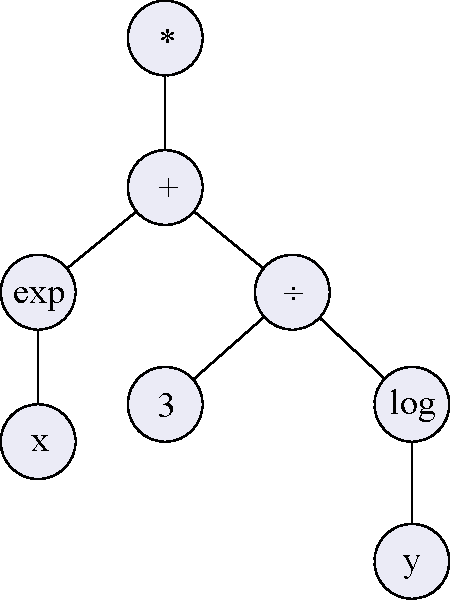
\includegraphics[scale=0.8]{tree.pdf}
\caption{Tree $\Gamma_f$ for expression $f = e^x + \frac{3}{\log(y)}$}
\label{fig::tree}
\end{figure}

\subsection{Meta learning problem}
This study explores the approach of meta learning for finding models of base problems.
Denote by $\mathfrak{D} = \{D_i = (\mathbf{X}_i, \mathbf{y}_i), f_i\}_{i=1}^m$ the data for the meta learning problem (meta learning dataset).

The following conditions are satisfied for meta learning dataset $\mathfrak{D}$:
\begin{itemize}
  \item $\text{dom}(\mathbf{x}_i) = \text{dom}(\mathbf{x}_j) \ \forall i, j$ (all $\mathbf{X}$ share the same domain),
  \item $f_i$ is an optimal model for the base problem $D_i$ in a model space $\mathfrak{F}$:
\end{itemize}
\begin{equation}
  f_i = \argmin_{f \in \mathfrak{F}} \text{MSE} (\mathbf{y}_i, f_i(\mathbf{X}_i)),
\end{equation}
where
\begin{equation}
  \text{MSE}(\mathbf{y}, \hat{\mathbf{y}}) = \frac{1}{l} \sum_{j=1}^{l} (y_j - \hat{y}_j)^2
\end{equation}
is a mean squared error of the model on the base problem.

Given the meta learning dataset $\mathfrak{D}$, the goal is to find an optimal meta learning model $\mathfrak{g}: D \rightarrow f$ which minimizes the error among all base problems:
\begin{equation}
  \mathfrak{g} = \argmin_{\mathfrak{g}} \mathcal{L}(\mathfrak{g}, \mathfrak{D}),
\end{equation}
\begin{equation}
  \label{error}
  \mathcal{L}(\mathfrak{g}, \mathfrak{D}) = \frac{1}{m} \sum_{i=1}^m \text{MSE}(\mathbf{y}_i, \mathfrak{g}(D_i)(\mathbf{X}_i)).
\end{equation}
\newpage

\section{Meta learning approach}
In this section we show how to find meta model $\mathfrak{g}$ which generalizes well to new base problems. We present framework for generating non-parametric models $f$ and then expand it to allow parameters.

\subsection{Choice of representation}
The meta learning function is a mapping between base problems $D$ and the space of mathematical expressions $\mathfrak{F}$. In order to define such mapping, define a suitable representation of base problem and its model.
\paragraph{Base problem representation}
Denote by $\mathbf{d} = [\text{vec}(\mathbf{X}), \mathbf{y}]^T$ the vector representation of a base problem $D$. This vector is a concatenation of vectorized feature matrix $\mathbf{X}$ and target vector $\mathbf{y}$

\textbf{Assumption 1.} \textit{All information needed for a generation of a model $f$ for a base problem $D$ is encoded in its representation vector $\mathbf{d}$.}

\paragraph{Model representation}
There are three ways to represent a model $f$:
\begin{itemize}
  \item the mathematical expression of $f$,
  \item the tree $\Gamma_f$, corresponding to the model $f$,
  \item the adjacency matrix $\mathbf{Z}_f$, corresponding to the tree $\Gamma_f$.
\end{itemize}

The third way allows a vectorized representation of a model $f$, it is selected for the proposed method of model generation.
Therefore, the meta model $\mathfrak{g}: \mathbb{R}^n \rightarrow \mathbb{Z}$ is a mapping between vector representations of a model and the space $\mathbb{Z}$ of valid adjacency matrices of mathematical expressions.

\subsection{Meta model decomposition}
The matrix $Z_f$, predicted with meta model $\mathfrak{g}$, has to satisfy all conditions on a tree $\Gamma_f$, listed in section \ref{sec::tree}.
Therefore, the construction of direct mapping $\mathfrak{g}$ is infeasible.
The proposed method is to decompose the meta model into two stages:
\begin{equation}
  \mathbf{Z}_f = \mathfrak{g}(\mathbf{d}) = g_\text{rec}(g_\text{clf}(\mathbf{d})),
\end{equation}
where $g_\text{rec}$ is a recovery function and $g_\text{clf}$ is a classification function.

\paragraph{Classification function}
$g_\text{clf}: \mathbb{R}^n \rightarrow \mathbb{P}$ is a mapping between vector representations of a model and the space $\mathbb{P}$ of matrices of edge probabilities. Therefore,
\begin{equation}
  g_\text{clf}(\mathbf{d}) = \mathbf{P}_f,
\end{equation}
where $\mathbf{P}_f$ is a matrix of probabilities of edges in the tree $\Gamma_f$. $g_\text{clf}$ is a multi label classification algorithm, which predicts the probability $p_{ij} \in [0, 1]$ that there is an edge between vertices $v_i$ and $v_j$ for any pair of vertices in the tree $\Gamma_f$.

\paragraph{Recovery function}
 $g_\text{rec}: \mathbb{P} \rightarrow \mathbb{Z}$ is a mapping between the space $\mathbb{P}$ of matrices of edge probabilities and the space $\mathbb{Z}$ of valid matrices for mathematical expressions. $g_\text{rec}$ is a nonparametric algorithm which selects the edges for $\Gamma_f$, based on their probabilities from $\mathbf{P}_f$. The resulting tree satisfies conditions from section \ref{sec::tree}.

In this study we propose two different methods for tree recovery, based on greedy strategy and dynamic programming approaches.

\subsection{Greedy algorithm}
The first approach to matrix recovery is to use greedy strategy.
The algorithm 1 builds the tree step-by-step, adding edges with highest probability, starting from the root. The algorithm stops early if the depth of the tree reached defined limit. Therefore the following corollary is true.

\textbf{Corollary 1.}\textit{The greedy algorithm of matrix recovery has $O(1)$ complexity.}

The corollary 1 also implies that the greedy algorithm is the fastest way to recover tree from matrix of edge probabilities.


\begin{algorithm}[!ht]
\caption{Decoys generation procedure}
 \KwData{Matrix of the edge probabilities $\mathbf{P}$}
 \KwResult{Recovered model $f$}
 Initialize set of open vertices $S = \{*\}$\;
 \While{$ S \neq \emptyset$ and maximum complexity is not reached}{
  Extract vertex $i$ from $S$\;
  \If{$i$ is a variable}
  {
	\textbf{continue}\;
  }
  Select vertex $j=\argmax_j \mathbf{P}_{ij}$ (the vertex with the highest edge probability)\;
  Grow tree $f$ with edge $(i, j)$\;
  Add $j$ to the set of open vertices $S$\;
}
\end{algorithm}
\newpage
\subsection{Dynamic programming}
The second approach to matrix recovery is to use dynamic programming approach.
In this case on each step the of the algorithm 2 the problem of tree recovery is divided into smaller problem, which are combined to maximize some score $s(f)$.

There are two possible variants for score function $s(f)$:
\begin{itemize}
	\item $s(f) = \prod\limits_{e \in f} P_{e}$, i.e. the product of all edges probabilities (tree likelihood);
	\item $s(f) = \frac{1}{n}\sum\limits_{e \in f} P_{e}$, i.e. score is the average probability of the edges in the tree.
\end{itemize}
Intuitively, the former score function penalizes deep trees heavily, while the latter allows more complex models.

It is straightforward to show that algorithm 2 uses dynamic programming approach.

\textbf{Bellman's principle of optimality.} \textit{An optimal policy has the property that whatever the initial state and initial decision are, the remaining decisions must constitute an optimal policy with regard to the state resulting from the first decision.}

\textbf{Corollary.} \textit{Algorithm 2 satisfies Bellman's principle of optimality.}\\
\textit{Proof.} Consider arbitrary step of the algorithm. The initial state is a given tree $f'$ and initial decisions are vertex choices that lead to the construction of such tree.

Then the algorithm finds the best subtree given the initial state, satisfying principle of optimality. $\blacksquare$

\begin{algorithm}[!ht]
\caption{Recursive procedure $r(\mathbf{P}, f, i)$ for dynamic programming}
	\KwData{Matrix of the edge probabilities $\mathbf{P}$; current tree $f$; leaf vertex~$i$ of $f$}
	\KwResult{$\hat{f}, s(\hat{f})$. \enspace $\hat{f}$ is the best continuation of $f$ and has $i$ as its root.}
	\If{$i$ is a variable}
	 {\Return$i$, $1$}
	\For{each unused vertex and variable $j$}{
	$f_j = f + (i, j)$ \enspace (grow tree $f$ with the edge $(i, j)$)\;
	$\hat{f_j}, s(\hat{f_j}) = r(P, f_j, j)$ \enspace (find optimal continuation for $f_j$)\;
	}
	$\hat{f} = \argmax_{f_j} s(\hat{f_j} + (i, j))$ \enspace (select optimal continuation for $f$)\;
	$s(\hat{f}) = \max_{f_j} s(\hat{f_j} + (i, j))$\;
	\Return $\hat{f}, s(\hat{f})$
\end{algorithm}

\subsection{Parametrization}
In previous sections the method for building mathematical expressions was introduced.
Next step is to expand it to parametric case.
It allows the method to work on real data and provides better approximation quality.

Suppose the nonparametric mathematical expression $f$ is an output of some recovery algorithm from previous sections. From the section \ref{base},
\begin{equation}
  f = g_1 \circ g_2 \circ \cdots \circ g_k,
\end{equation}
where $g_i$ is a nonparametric primitive function. To parametrize model $f$, let us parametrize each primitive function $g_i$:
\begin{equation}
  g_i(\mathbf{x}, \alpha_{i1}, \alpha_{i0}) = \alpha_{i1}g_i(\mathbf{x}) + \alpha_{i0}
\end{equation}
The parameters of model $f$ are the parameters of its primitive functions:
\begin{equation}
  f(\mathbf{x}) \rightarrow f(\mathbf{x}, \bm{\alpha})
\end{equation}
The resulting function is differentiable and the optimal parameters are found using gradient descent.

The proposed method is described in algorithm 3 and algorithm 4.

\begin{algorithm}[!ht]
\caption{Training procedure}
	\KwData{Meta learning dataset $\mathfrak{D} = \{D_i = (\mathbf{X}_i, \mathbf{y}_i), f_i\}_{i=1}^m$}
	\KwResult{Optimal meta model $\mathfrak{g}$}
	\For{each base problem $D_i$}{
  remove parameters (constants) from model $f_i$\;
  represent model $f_i$ with adjacency matrix $\mathbf{Z}_{f_i}$ of its corresponding tree $\Gamma_{f_i}$\;
  represent base problem $D_i$ with a vector $\mathbf{d}_i = [\text{vec}(\mathbf{X}_i), \mathbf{y}_i]^T$
  }
  train multi label classifier $g_\text{clf}$ on the set of pairs $\{(\mathbf{d}_i, \mathbf{Z}_{f_i})\}$\;
\end{algorithm}

\begin{algorithm}[!ht]
\caption{Inference procedure}
	\KwData{Base problem $D = (\mathbf{X}, \mathbf{y})$}
	\KwResult{Optimal model $f$}
  represent base problem $D$ with a vector $\mathbf{d} = [\text{vec}(\mathbf{X}), \mathbf{y}]^T$\;
  predict probability matrix $\mathbf{P}_f: \ \mathbf{P}_f = g_\text{clf}(\mathbf{d})$\;
  recover adjacency matrix $\mathbf{Z}_f: \ \mathbf{Z}_f = g_\text{rec}(\mathbf{P}_f)$\;
  parametrize the model $f \rightarrow f(\bm{\alpha})$\;
  find optimal $\bm{\alpha}$ using gradient descent\;
\end{algorithm}

\newpage

\section{Computational experiment}
The proposed method was tested on generated and real data.
The goal of the experiment is to compare variations of the algorithm on synthetic data, and then compare its performance with symbolic regression on the real data.
All the experiments were conducted on 1-D time series data.
\subsection{Synthetic data}
The goal of this experiment is to prove that meta learning method works and test different variations of it.
For all the experiments in this study we chose the following properites of the models:
\begin{itemize}
  \item the depth of the tree doesn't exceed 10,
  \item Binary operators: $+, \times$,
  \item Unary operators: $\sin, \cos, \exp, \log, \frac{1}{x}, \sqrt{x}, x^2$.
\end{itemize}

The full scheme of generating synthetic data can be found in the algorithm 5.
The difference between parametric and nonparametric setup is the presence of the parameters in the tree on the step \ref{param}.

\begin{algorithm}[!ht]
\caption{Generate data for synthetic experiment}
	\KwResult{Synthetic dataset $\mathfrak{D}$}
  \For{$i = 1, \dots, m$}{
  sample $n$ points $\mathbf{x} = \{x_i\}_{k=1}^n$ uniformly from $[-5, 5]$\;
  create random tree $\Gamma_{f_i}$ (start building tree from root ``*'', sampling operators or variables with equal probabilities)\;
  \label{param}
  generate target variable $\mathbf{y}$ and add gaussian noise: \ $y_k = f_i(x_k) + \mathcal{N}(0, 0.05)$\;
  base problem $D_i = (\mathbf{x}, \mathbf{y})$\;
  add problem-model pair $(D_i, f_i)$ to the meta learning dataset $\mathfrak{D}$\;
  }
  split dataset $\mathfrak{D}$ into train $\mathfrak{D}_\text{train}$ and test $\mathfrak{D}_\text{test}$\;
\end{algorithm}


\subsubsection{Nonparametric approach}
In this experiment the size of the dataset $\mathfrak{D}$ is 5000, $|\mathfrak{D}_\text{train}| = 4500$, $|\mathfrak{D}_\text{test}| = 500$. Greedy algorithm and two variations of dynamic programming were tested as recovery functions.
Random forest, neural network with 2 hidden layers and logistic regression were variations of classification functions.

The examples of generated models for the test set are shown on the figure \ref{fig::nonparametric}.
The red dots are generated data and colored lines are models, obtained with various recovery functions.
Random forest was used as a classification algorithm for generation of these examples.
\begin{figure}[!ht]
\centering
\begin{subfigure}{0.48\textwidth}
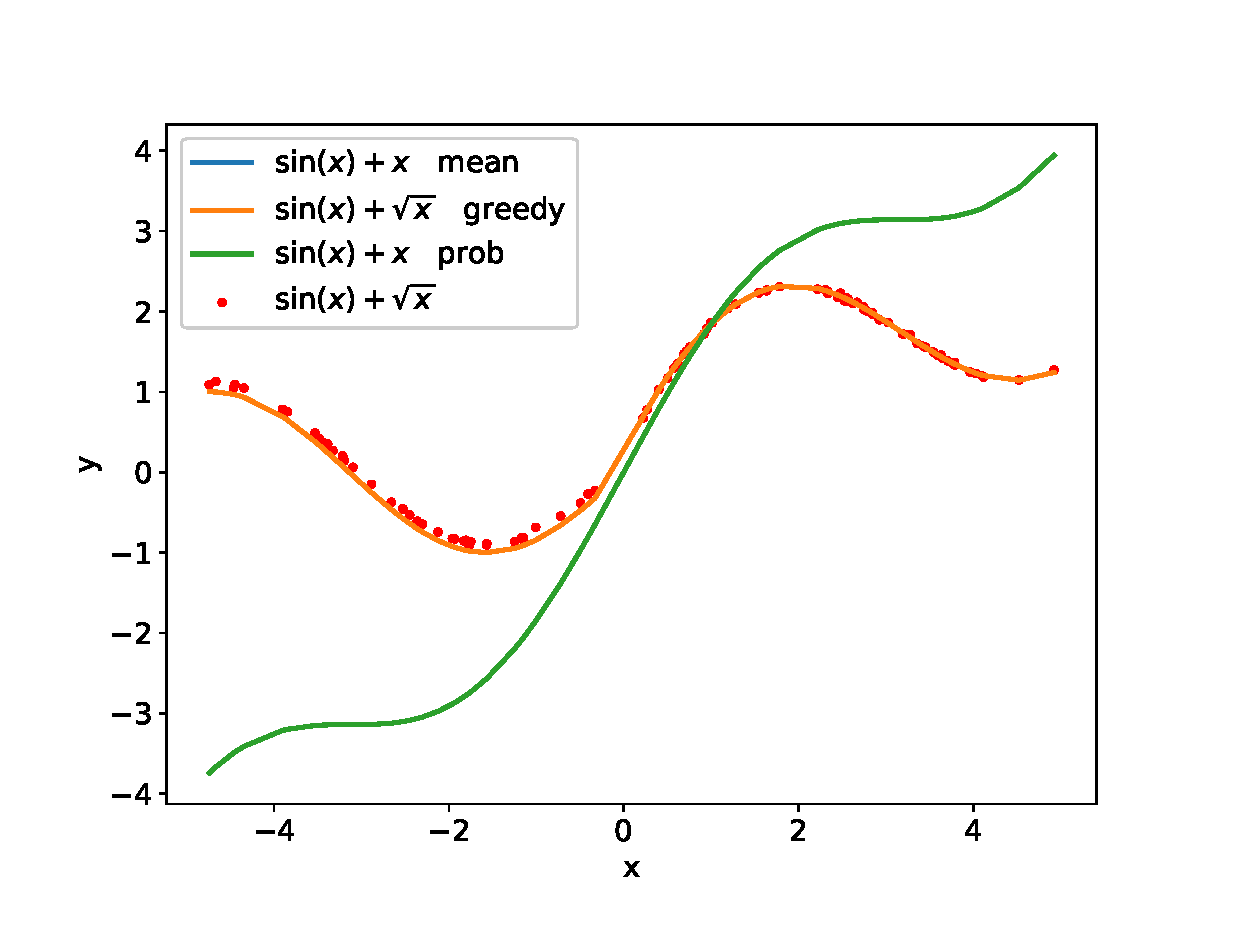
\includegraphics[width=\textwidth]{_non_param_1.eps}
\caption{}
\label{fig::_non_param_1}
\end{subfigure}
~
\begin{subfigure}{0.48\textwidth}
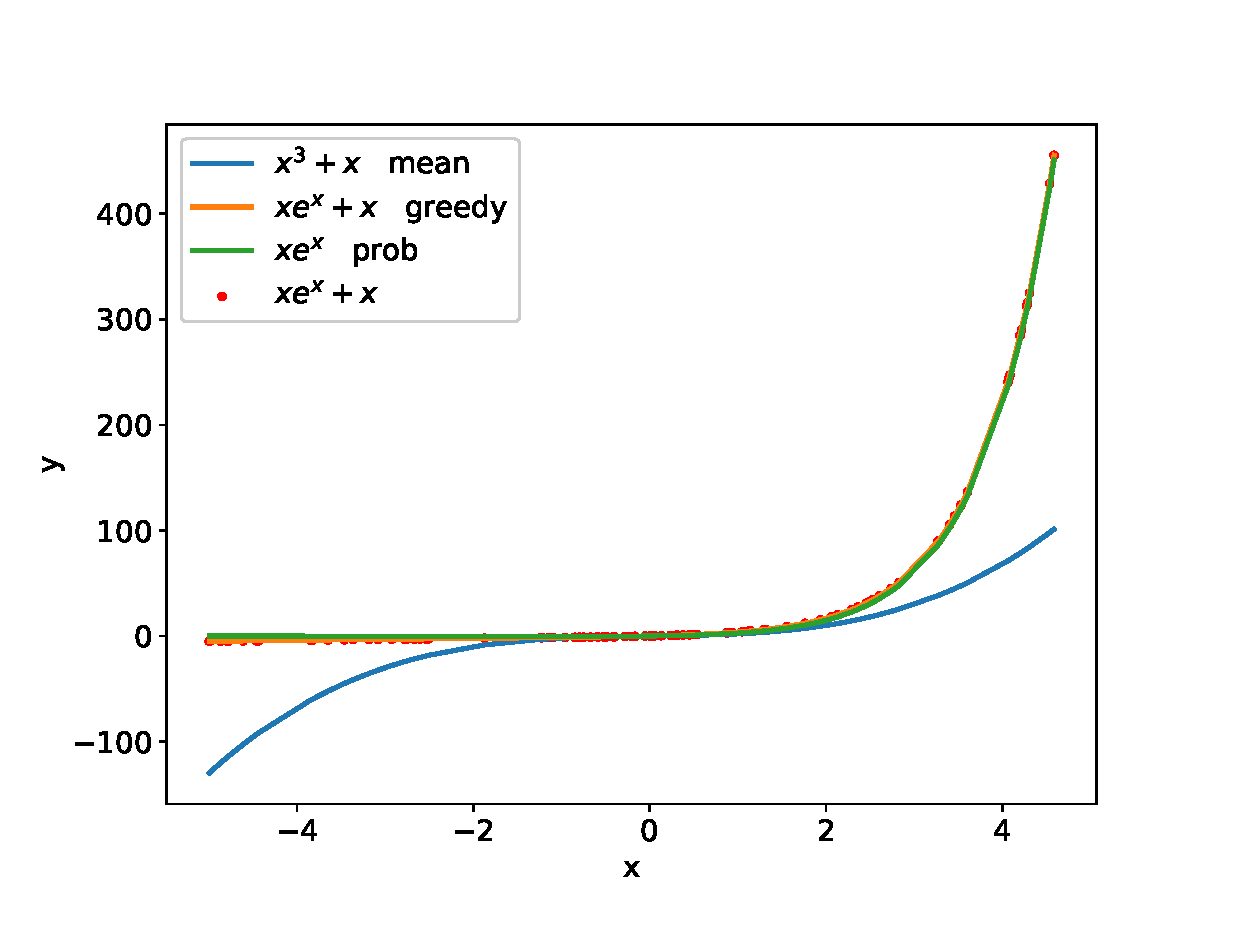
\includegraphics[width=\textwidth]{_non_param_2.eps}
\caption{}
\label{fig::_non_param_2}
\end{subfigure}
\\
\begin{subfigure}{0.48\textwidth}
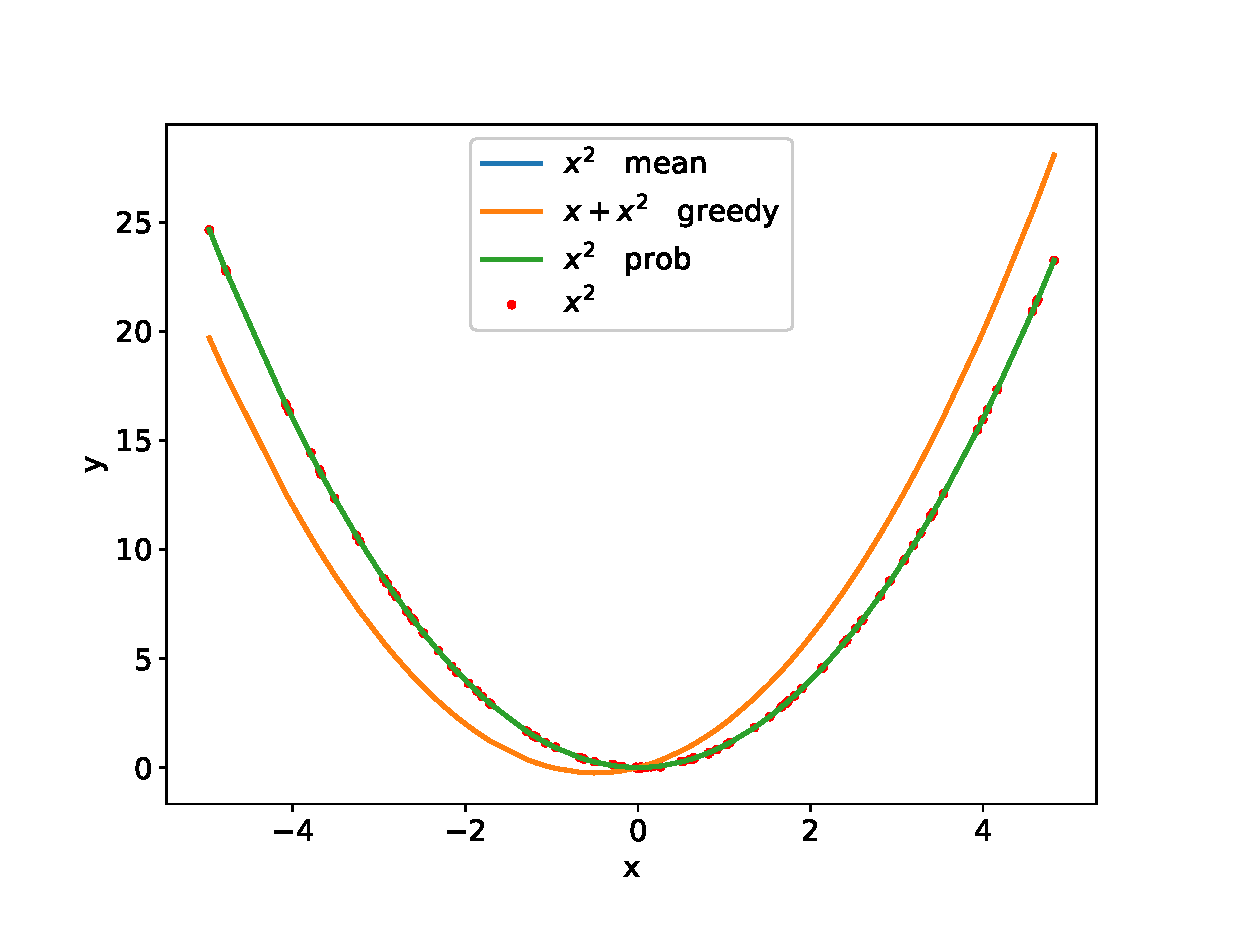
\includegraphics[width=\textwidth]{_non_param_3.eps}
\caption{}
\label{fig::_non_param_3}
\end{subfigure}
~
\begin{subfigure}{0.48\textwidth}
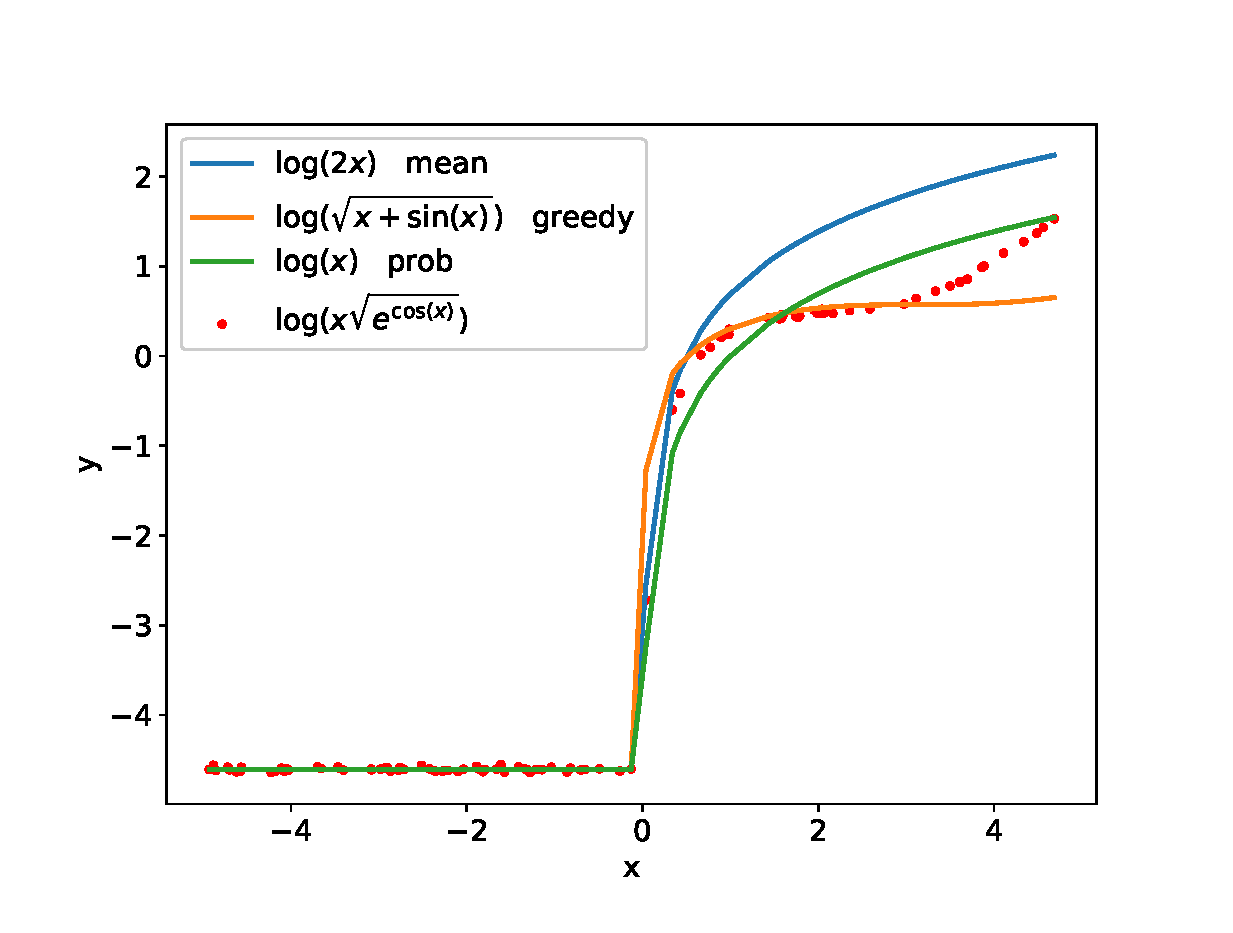
\includegraphics[width=\textwidth]{_non_param_4.eps}
\caption{}
\label{fig::_non_param_4}
\end{subfigure}
\caption{Performance of nonparametric approach on the test set.}
\label{fig::nonparametric}
\end{figure}

These examples shows that proposed method not only approximates data well, but also recovers the structure of the model correctly in most cases.
This observation proves, that in parametric case we will achieve high quality not because parameters tuning, but because of correct structure prediction.
Full results are shown in the table \ref{table-nonparam}.
The numbers in the table is an error of meta model on the test set, as defined in (\ref{error}).
Random forest is the classification method of highest quality in our experiments.
As expected the performance of greedy algorithm as a recovery function is worse than dynamic programming.

\begin{table}[!ht]
\centering
\caption{Results in a nonparametric case.}
\label{table-nonparam}
\begin{tabular}{c|c|c|c|}
\cline{2-4}
& \textit{Random Forest} & \textit{Neural network} & \textit{Logistic regression} \\ \hline
\multicolumn{1}{|c|}{\textbf{Greedy algorithm}}      & 5.45                   & 5.81           & 6.3                          \\ \hline
\multicolumn{1}{|c|}{\textbf{DP (tree likelihood)}}  & 5.41                   & 5.65           & 5.97                         \\ \hline
\multicolumn{1}{|c|}{\textbf{DP (mean probability)}} & \textbf{5.32}                   & 5.72           & 6.12                         \\ \hline
\end{tabular}
\end{table}

\subsubsection{Parametric approach}
The setup of the experiment in parametric settings is the same, as in nonparametric case.
The results of the experiment are shown in the table \ref{table-param}.

\begin{table}[!ht]
\centering
\caption{Results in a parametric case.}
\label{table-param}
\begin{tabular}{c|c|c|c|}
\cline{2-4}
& \textit{Random Forest} & \textit{Neural network} & \textit{Logistic regression} \\ \hline
\multicolumn{1}{|c|}{\textbf{Greedy algorithm}}      & 7.02                   & 7.13           & 7.35                          \\ \hline
\multicolumn{1}{|c|}{\textbf{DP (tree likelihood)}}  & \textbf{6.88}                   & 6.93           & 7.01                         \\ \hline
\multicolumn{1}{|c|}{\textbf{DP (mean probability)}} & 6.92                   & 6.94           & 6.99                         \\ \hline
\end{tabular}
\end{table}

Our conclusions from nonparametric case stay true in parametric case as well.
Random forest is the best classifier, and greedy algorithm has larger error than dynamic programming on the test set.
The examples of models for the test set, obtained from random forest and tree likelihood recovery function are shown in the figure \ref{fig::parametric}.
Red dots are ground truth data and blue line is a predicted model.
\newpage
\begin{figure}[!ht]
\centering
\begin{subfigure}{0.48\textwidth}
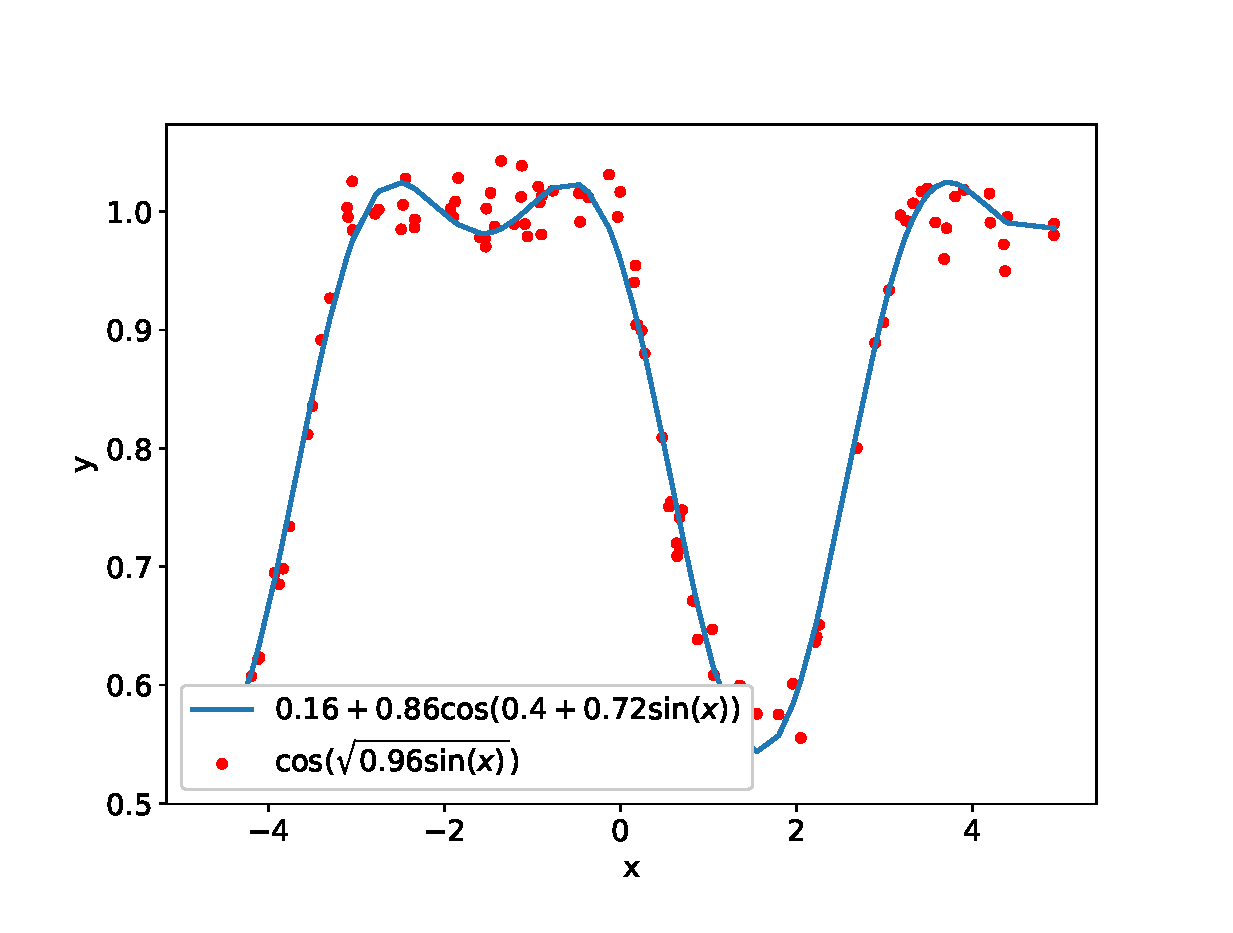
\includegraphics[width=\textwidth]{_res_param_1.eps}
\caption{}
\label{fig::_res_param_1}
\end{subfigure}
~
\begin{subfigure}{0.48\textwidth}
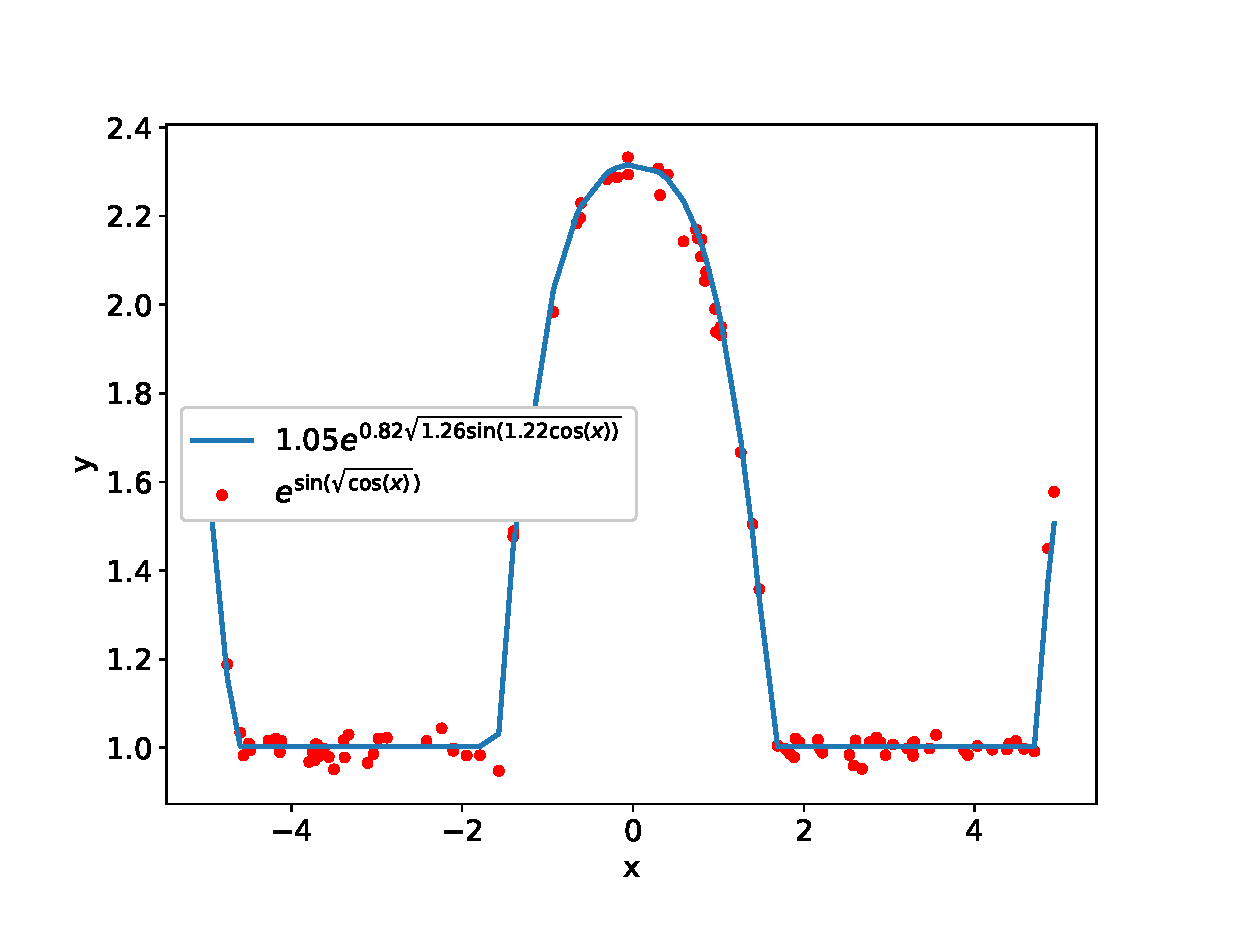
\includegraphics[width=\textwidth]{_res_param_2.eps}
\caption{}
\label{fig::_res_param_2}
\end{subfigure}
\\
\begin{subfigure}{0.48\textwidth}
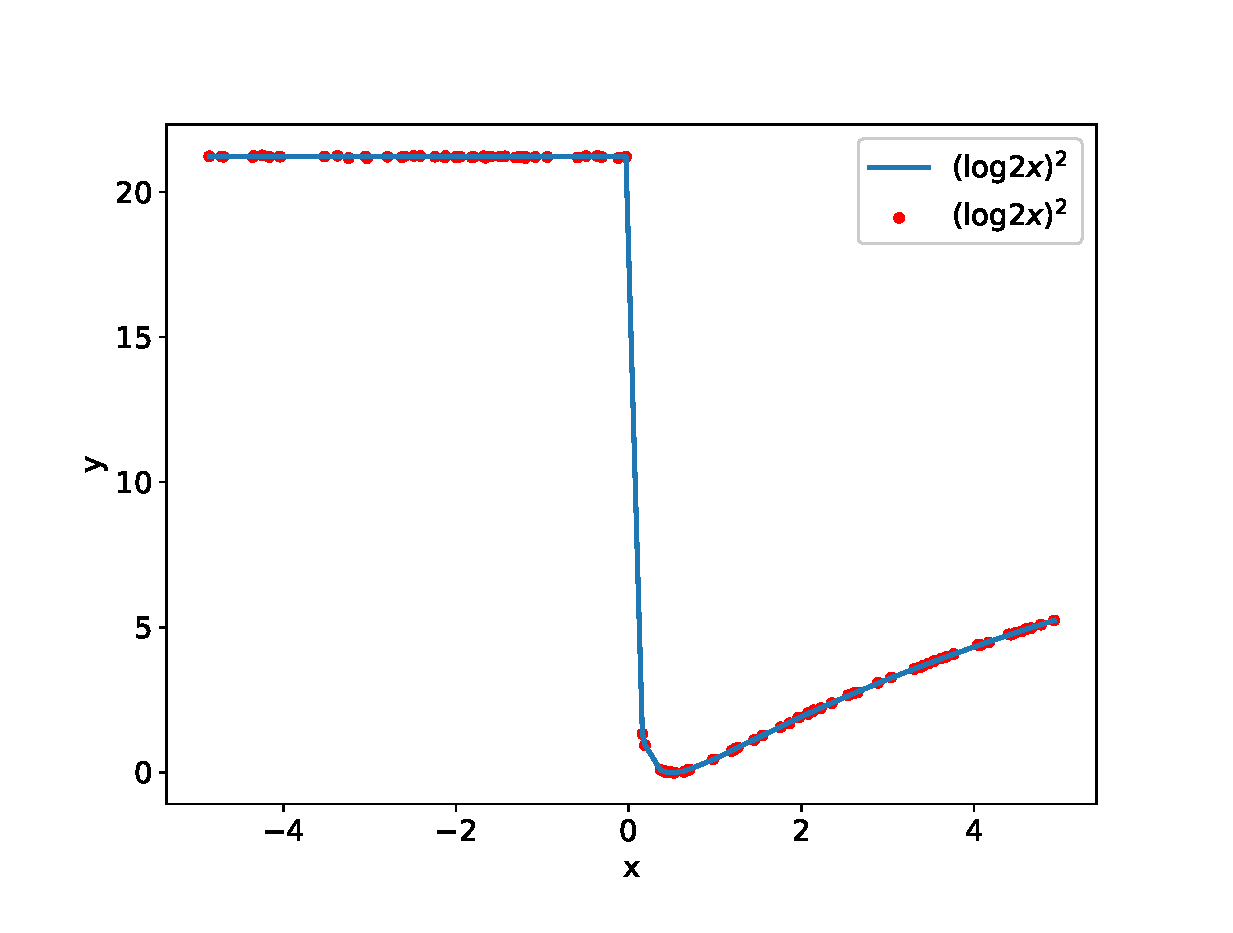
\includegraphics[width=\textwidth]{_res_param_3.eps}
\caption{}
\label{fig::_res_param_3}
\end{subfigure}
~
\begin{subfigure}{0.48\textwidth}
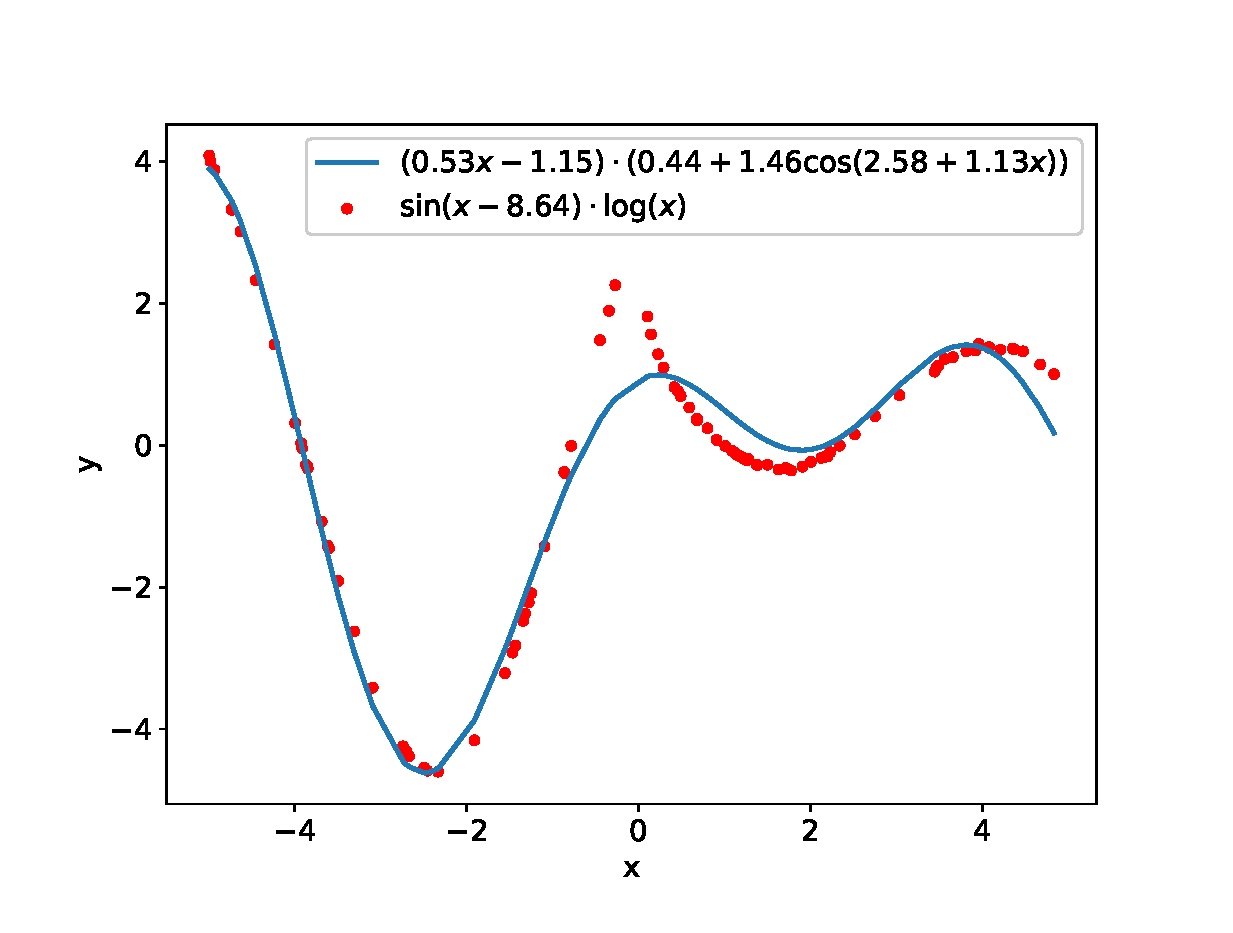
\includegraphics[width=\textwidth]{_res_param_4.eps}
\caption{}
\label{fig::_res_param_4}
\end{subfigure}
\caption{Performance of parametric approach on the test set.}
\label{fig::parametric}
\end{figure}

These examples show that parametric method correctly recovers underlying model from the data.
Even if it fails to predict the structure exactly, introduction of parameters allows model to have low error.
In some cases the structure and the parameters are recovered exactly.

\subsection{Real data}
The goal of the experiment on the real data is to show that the proposed method is faster than symbolic regression, without significant drop in quality of the predicted models.
The real experiment is conducted on two time series datasets.

To compare the performance of meta model and symbolic regression, we need to fit the latter on each base problem.
The algorithm 6 shows the procedure for extracting meta learning dataset from real time series data.

\begin{algorithm}[!ht]
\caption{Generate data for real experiment}
	\KwResult{Real dataset $\mathfrak{D}$}
  \For{$i = 1, \dots, m$}{
  sample a segment of $n$ points from time series: $\mathbf{x} = \{x_i\}_{k=1}^n, \mathbf{y} = \{y_i\}_{k=1}^n$\;
  find the optimal approximating model $f_i$ for the segment using symbolic regression\;
  \label{symbolic}
  base problem $D_i = (\mathbf{x}, \mathbf{y})$\;
  add problem-model pair $(D_i, f_i)$ to the meta learning dataset $\mathfrak{D}$\;
  }
  split dataset $\mathfrak{D}$ into train $\mathfrak{D}_\text{train}$ and test $\mathfrak{D}_\text{test}$\;
\end{algorithm}

In this experiment we compare the quality of models obtained from meta model and from symbolic regression.
We also compare the time of finding optimal model on the step \ref{symbolic} and of inference procedure of meta model (algorithm 4).
The greedy algorithm is selected as a recovery function for the fastest inference of the proposed method.

\paragraph{Daily foreign exchange rates}
The dataset \cite{exchange-rates} contains time series of exchange rate between USD and foreign currency for the period from 31 December 1979 to 31 December 1998.
The time series contain 4770 data points.
Using algorithm 6 we generate $m=1000$ time series segments of length $n=100$. The size of the training set and test set is 900 and 100 accordingly.
The example of the time series segment and corresponding symbolic regression model are shown on figure \ref{fig::exchange}.

Mean squared error and mean inference speed of two approaches are shown in the table \ref{table-exchange}.
The proposed meta learning method provides 20x speedup of inference type in comparison with symbolic regression approach. Moreover, the models from meta model are marginally worse than those, obtained with symbolic regression.
\begin{figure}[!ht]
\centering
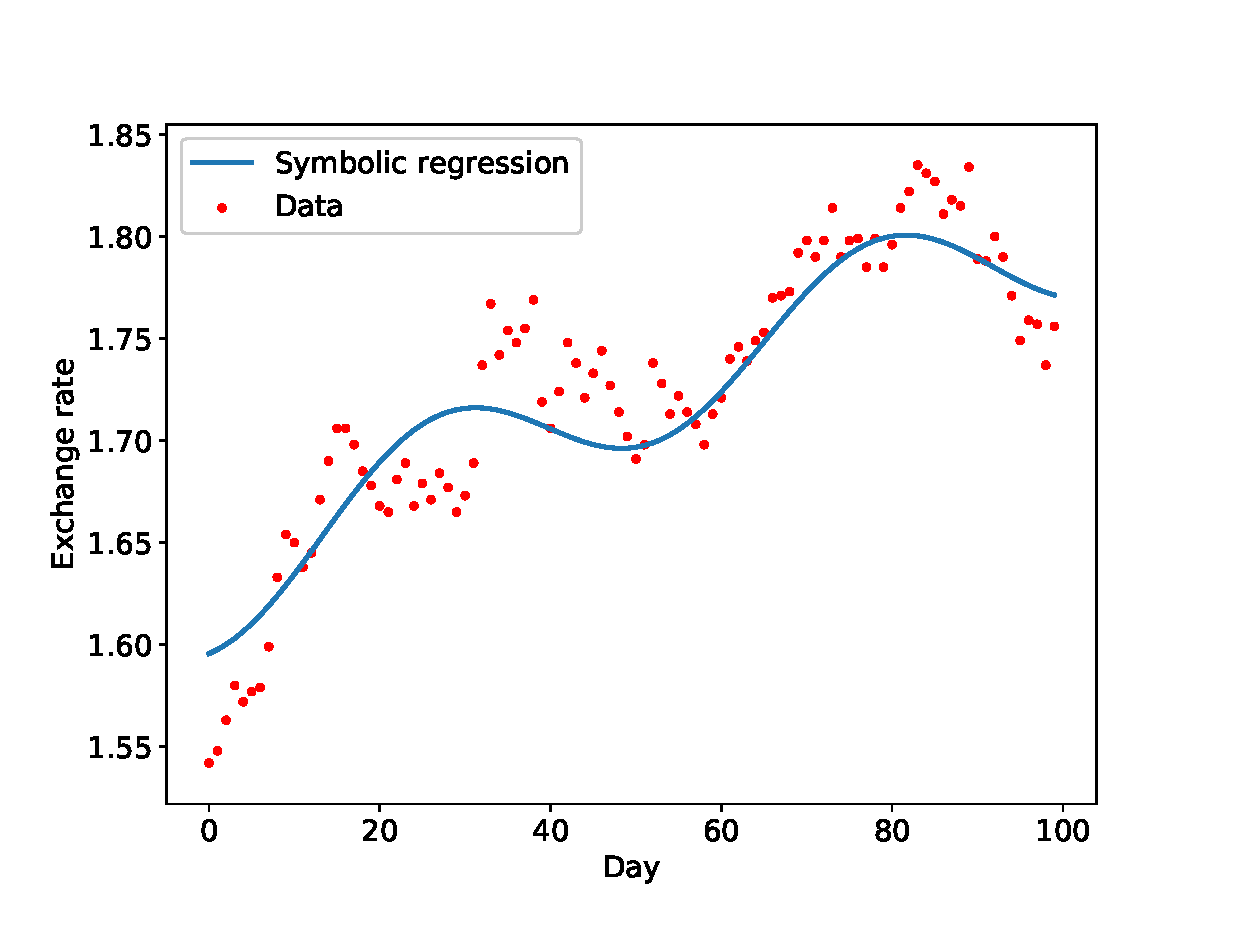
\includegraphics[scale=0.7]{exchange.eps}
\caption{Example of time series segment}
\label{fig::exchange}
\end{figure}

\begin{table}[!h]
\centering
\caption{Results comparison on exchange dataset}
\label{table-exchange}
\begin{tabular}{c|c|c|}
\cline{2-3}
                                                   & \textit{MSE} & Inference speed, sec. \\ \hline
\multicolumn{1}{|c|}{\textbf{Symbolic regression}} & 0.012        & 6.02                  \\ \hline
\multicolumn{1}{|c|}{\textbf{Meta model}}          & 0.014        & 0.28                  \\ \hline
\end{tabular}
\end{table}

\paragraph{Stock prices}
The dataset \cite{stock} contains time series of IBM common stock closing prices for the period from 2 Jan 1962 to 31 Dec 1965.
The time series contain 1008 data points.
Using algorithm 6 we generate $m=500$ time series segments of length $n=100$. The size of the training set and test set is 400 and 100 accordingly.
The example of the time series segment and corresponding symbolic regression model are shown on figure \ref{fig::stock}.

Comparison of the two approaches on the stock data is shown in \ref{table-stock}.
The speedup and the performance of the proposed method is very similar to the result on the exchange dataset.
Meta learning approach gives great speedup without big sacrifies in a quality of the models.
\newpage
\begin{figure}[!ht]
\centering
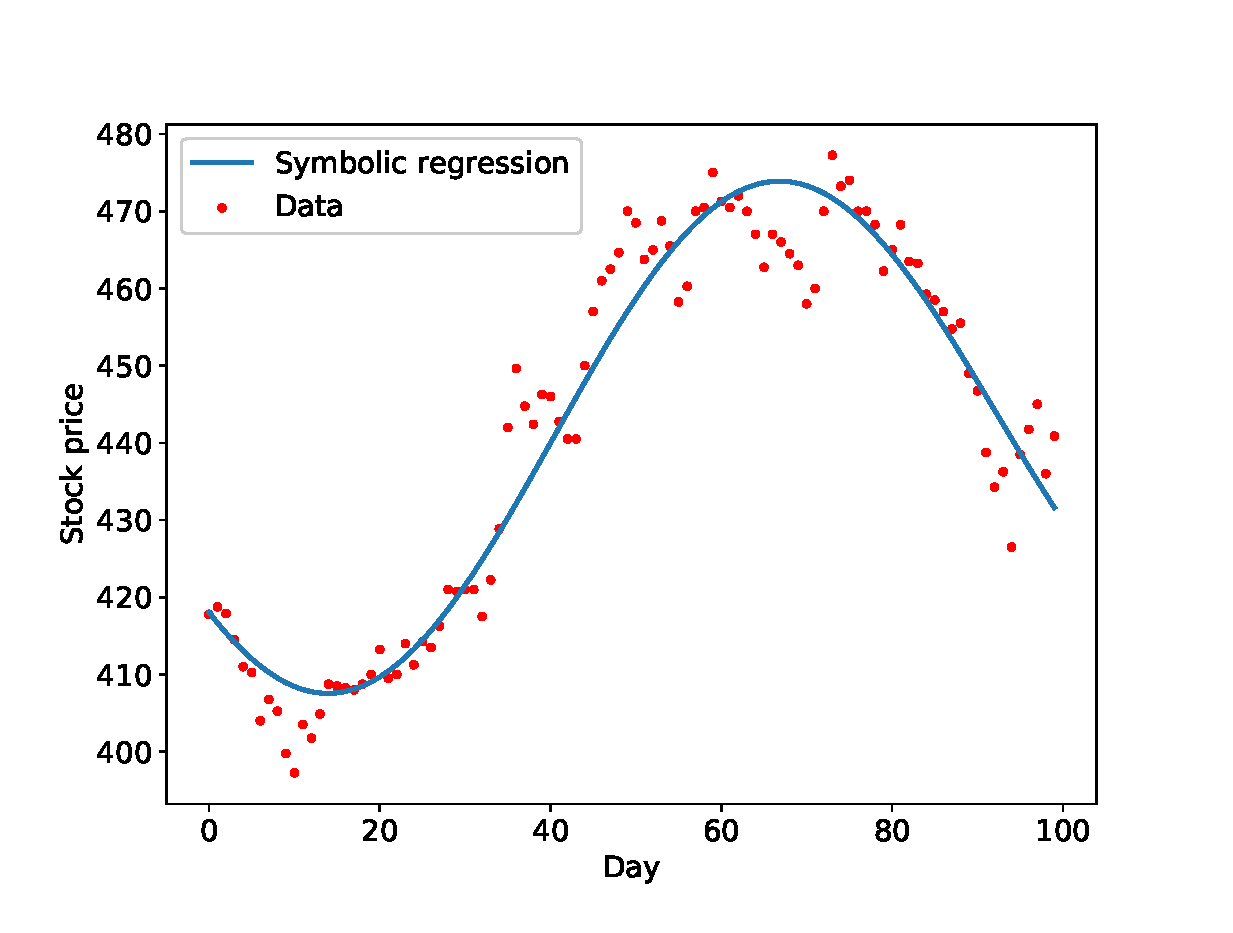
\includegraphics[scale=0.7]{stock.eps}
\caption{Example of time series segment}
\label{fig::stock}
\end{figure}

\begin{table}[!ht]
\centering
\caption{Results comparison on stock price dataset}
\label{table-stock}
\begin{tabular}{c|c|c|}
\cline{2-3}
                                                   & \textit{MSE} & Inference speed, sec. \\ \hline
\multicolumn{1}{|c|}{\textbf{Symbolic regression}} & 3.13        & 6.34                  \\ \hline
\multicolumn{1}{|c|}{\textbf{Meta model}}          & 3.22        & 0.31                  \\ \hline
\end{tabular}
\end{table}


\newpage

\section{Conclusion}

\newpage
\bibliographystyle{unsrt}
\bibliography{lib.bib}
\end{document}
